\subsection{Oversigt}

Vi har valgt at tage Physical View med fordi det beskriver hvordan de forskellige del-systemer er forbundne, og hvilke veje kommunikationen mellem dem foregår.

\begin{figure}[htb]
    \centering
    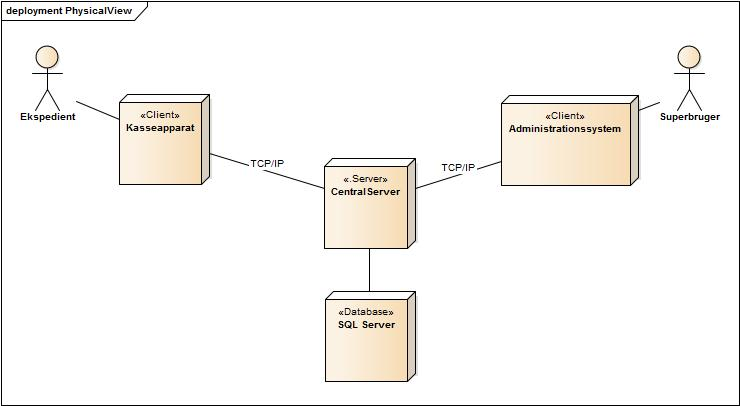
\includegraphics[width=0.8\textwidth]{Systemarkitektur/PhysicalView/Billeder/PhysicalView.jpg}
    \caption{Physical view af systemet}
    \label{fig:physicalview}
\end{figure}

Alle del-systemer kommunikerer vha. TCP/IP~\cite{TCPIP} sockets, og systemerne kan derfor eksekvere og kommunikere asynkront på forskellige fysiske maskiner. \gls{Eks} og \gls{SB} kan derfor tilgå hvert deres system på samme tid fra forskellige maskiner.